\documentclass[11pt]{article}
\usepackage[utf8]{inputenc}
\usepackage{geometry}
\usepackage{amsmath}
\usepackage{amsfonts}
\usepackage{amssymb}
\usepackage{graphicx}
\usepackage{hyperref}
\usepackage{xcolor}
\usepackage{listings}
\usepackage{enumitem}
\usepackage{array}
\usepackage{booktabs}
\usepackage{longtable}
\usepackage{glossaries}
\usepackage{tikz}
\usetikzlibrary{positioning, arrows.meta, shapes}

% Page geometry
\geometry{a4paper, margin=1in}

% Hyperref setup
\hypersetup{
    colorlinks=true,
    linkcolor=blue,
    urlcolor=blue,
    citecolor=blue
}

% Define YAML language for listings
\lstdefinelanguage{yaml}{
    sensitive=true,
    keywords={true,false,null,y,n},
    keywordstyle=\color{blue}\bfseries,
    basicstyle=\ttfamily\small,
    comment=[l]{\#},
    commentstyle=\color{green!40!black},
    stringstyle=\color{red},
    morestring=[b]',
    morestring=[b]",
    identifiersstyle=\color{black},
    literate=*{:}{: }1
}

% Code listing style
\lstdefinestyle{pythonstyle}{
    language=Python,
    basicstyle=\ttfamily\small,
    commentstyle=\color{green!40!black},
    keywordstyle=\color{blue},
    stringstyle=\color{red},
    showstringspaces=false,
    numbers=left,
    numberstyle=\tiny,
    numbersep=5pt,
    breaklines=true,
    frame=single
}

\lstdefinestyle{cppstyle}{
    language=C++,
    basicstyle=\ttfamily\small,
    commentstyle=\color{green!40!black},
    keywordstyle=\color{blue},
    stringstyle=\color{red},
    showstringspaces=false,
    numbers=left,
    numberstyle=\tiny,
    numbersep=5pt,
    breaklines=true,
    frame=single
}

\lstdefinestyle{bashstyle}{
    language=bash,
    basicstyle=\ttfamily\small,
    commentstyle=\color{green!40!black},
    keywordstyle=\color{blue},
    stringstyle=\color{red},
    showstringspaces=false,
    numbers=left,
    numberstyle=\tiny,
    numbersep=5pt,
    breaklines=true,
    frame=single
}

\lstdefinestyle{yamlstyle}{
    language=yaml,
    basicstyle=\ttfamily\small,
    keywordstyle=\color{blue}\bfseries,
    commentstyle=\color{green!40!black},
    stringstyle=\color{red},
    showstringspaces=false,
    numbers=left,
    numberstyle=\tiny,
    numbersep=5pt,
    breaklines=true,
    frame=single
}

% Title
\title{The Complete MLOps Lifecycle: \\ From Conceptual Architecture to Production}
\author{Deep Learning Engineering}
\date{\today}

% Glossary entries
\newglossaryentry{mlops}{
    name=MLOps,
    description={Machine Learning Operations, a set of practices that aims to deploy and maintain machine learning models in production reliably and efficiently}
}

\newglossaryentry{kubernetes}{
    name=Kubernetes,
    description={An open-source container orchestration platform that automates the deployment, scaling, and management of containerized applications. Often abbreviated as K8s}
}

\newglossaryentry{docker}{
    name=Docker,
    description={A platform for developing, shipping, and running applications in containers. Containers package software with its dependencies, ensuring consistency across environments}
}

\newglossaryentry{container}{
    name=Container,
    description={A lightweight, standalone, executable package that includes everything needed to run software: code, runtime, system tools, libraries, and settings}
}

\newglossaryentry{cuda}{
    name=CUDA,
    description={Compute Unified Device Architecture. A parallel computing platform and programming model created by NVIDIA for general computing on GPUs}
}

\newglossaryentry{cnn}{
    name=CNN,
    description={Convolutional Neural Network. A class of deep neural networks most commonly applied to analyzing visual imagery}
}

\newglossaryentry{tensorrt}{
    name=TensorRT,
    description={NVIDIA's high-performance deep learning inference optimizer and runtime engine that delivers low latency and high throughput for deployment}
}

\newglossaryentry{onnx}{
    name=ONNX,
    description={Open Neural Network Exchange. An open format to represent machine learning models, allowing interoperability between different frameworks}
}

\newglossaryentry{xla}{
    name=XLA,
    description={Accelerated Linear Algebra. A domain-specific compiler for linear algebra that optimizes TensorFlow and JAX computations}
}

\newglossaryentry{kubeflow}{
    name=Kubeflow,
    description={A machine learning toolkit for Kubernetes that makes deploying and managing ML workflows on Kubernetes simpler, portable, and scalable}
}

\newglossaryentry{pytorch}{
    name=PyTorch,
    description={An open-source machine learning framework developed by Facebook's AI Research lab, known for its dynamic computational graphs}
}

\newglossaryentry{tensorflow}{
    name=TensorFlow,
    description={An open-source machine learning framework developed by Google, supporting both static and dynamic computational graphs}
}

\newglossaryentry{jax}{
    name=JAX,
    description={A Python library for accelerator-oriented array computation and large-scale machine learning, developed by Google Research}
}

\newglossaryentry{torchscript}{
    name=TorchScript,
    description={An intermediate representation of PyTorch models that can be run in high-performance environments without Python dependencies}
}

\newglossaryentry{ir}{
    name=Intermediate Representation,
    description={A data structure or code used internally by a compiler to represent source code, independent of the source language or target machine}
}

\newglossaryentry{kernel}{
    name=Kernel (CUDA),
    description={A function that is executed on a GPU device by multiple threads in parallel}
}

\newglossaryentry{pod}{
    name=Pod,
    description={The smallest and simplest Kubernetes object. Represents a single instance of a running process in a cluster, which can contain one or more containers}
}

\newglossaryentry{cluster}{
    name=Cluster,
    description={A set of machines, called nodes, that run containerized applications managed by Kubernetes}
}

\newglossaryentry{controlplane}{
    name=Control Plane,
    description={The container orchestration layer that exposes the API and interfaces to define, deploy, and manage the lifecycle of containers}
}

\newglossaryentry{etcd}{
    name=etcd,
    description={A consistent and highly-available key-value store used as Kubernetes' backing store for all cluster data}
}

\newglossaryentry{kubelet}{
    name=kubelet,
    description={An agent that runs on each Kubernetes node and ensures containers are running in a Pod}
}

\newglossaryentry{operatorfusion}{
    name=Operator Fusion,
    description={A compiler optimization that combines multiple operations into a single kernel to reduce memory transfers and improve performance}
}

\newglossaryentry{quantization}{
    name=Quantization,
    description={The process of reducing the numerical precision of a model's weights and activations from floating-point to lower-bit representations (e.g., FP32 to INT8)}
}

\newglossaryentry{pruning}{
    name=Pruning,
    description={The process of removing unnecessary or less important connections in a neural network to reduce model size and improve inference speed}
}

\newglossaryentry{distributedtraining}{
    name=Distributed Training,
    description={Training a single model across multiple devices or machines using data parallelism (splitting data) or model parallelism (splitting model)}
}

\newglossaryentry{modelregistry}{
    name=Model Registry,
    description={A centralized repository for storing, versioning, and managing machine learning models throughout their lifecycle}
}

\newglossaryentry{drift}{
    name=Model Drift,
    description={The degradation of model performance over time due to changes in the underlying data distribution (concept drift) or features (data drift)}
}

\newglossaryentry{serving}{
    name=Model Serving,
    description={The process of making a trained machine learning model available to make predictions, typically via an API endpoint}
}

\makeglossaries

\begin{document}

\maketitle

\begin{abstract}
This document provides a comprehensive overview of the complete MLOps lifecycle, from conceptual architecture design to production deployment and maintenance. It includes a granular breakdown of five distinct phases covering mathematical design, software representation, hardware compilation, execution, and deployment. A comprehensive glossary of key terms is also provided.
\end{abstract}

\tableofcontents
\newpage


\section{Introduction}

The journey of a deep learning model from a mere concept to a production system serving millions of users is a complex, multi-stage pipeline that parallels the construction and operation of a massive modern city. It begins in the architect's studio—the researcher's whiteboard—where the conceptual blueprint of a neural network is sketched out, defining its layers, connections, and mathematical foundations, much like an architect envisions the framework  of a skyscraper. This blueprint is then handed to engineers who translate it into actual building materials using frameworks like PyTorch or TensorFlow, writing Python code that defines the computational graph—analogous to ordering steel beams and concrete for the foundation. However, raw code, like raw materials, isn't ready for the construction site; it must be fabricated into standardized components through compilation into an intermediate representation such as TorchScript or ONNX. This step is akin to a steel factory prefabricating beams with precise measurements and connection points, ensuring they can be assembled efficiently. These prefabricated components are then shipped to the GPU construction site, where a master crane operator—the CUDA compiler—takes over, lifting each component (kernel) and placing it according to an optimized schedule (operator fusion and memory planning) to assemble the neural network with maximum efficiency, leveraging specialized tools like Tensor Cores that act as precision welding equipment. Once the skyscraper (the trained model) is complete, it must be transformed from a static structure into a functional building ready for occupancy. It is packaged into a self-contained, portable shipping container using Docker, encapsulating not just the model itself but all its dependencies—the furniture, plumbing, and electrical systems—ensuring it can run identically in any environment, whether on a developer's laptop or in a massive data center. But a single container is just one building; to create a resilient, scalable city district, you need a fleet of these containers working together. This is where Kubernetes enters as the city's harbor master and urban planner, orchestrating the deployment of thousands of containers, managing the flow of traffic (user requests) through load-balancing highways, automatically spinning up new buildings during rush hour (horizontal scaling), and seamlessly replacing any that develop structural issues (self-healing). The city doesn't stop evolving once built; continuous monitoring systems—like smart sensors throughout the metropolis—track performance metrics, detect when the underlying data landscape shifts (model drift), and trigger automated retraining pipelines (urban renewal projects) to keep the city's infrastructure responsive to changing conditions. From the architect's first sketch to a thriving, self-sustaining metropolis that adapts and grows, the MLOps lifecycle transforms abstract mathematical ideas into living, breathing intelligence that powers our world.

\section{Introduction to MLOps}

Machine Learning Operations (MLOps) is a set of practices that aims to deploy and maintain machine learning models in production reliably and efficiently. It extends DevOps principles to the machine learning lifecycle, addressing the unique challenges of model versioning, data versioning, training reproducibility, and model monitoring.

The complete MLOps lifecycle spans far beyond just training a model. It encompasses everything from the initial mathematical conception to the final user-facing application, with multiple layers of abstraction and optimization in between.

\section{Phase 1: Mathematical and Architectural Design}

\subsection{Conceptual Problem Definition}
Before any code is written, the problem must be clearly defined. This involves:
\begin{itemize}
    \item Identifying the business objective
    \item Defining input and output spaces
    \item Establishing success metrics (accuracy, precision, recall, F1, etc.)
    \item Understanding constraints (latency requirements, computational resources, privacy regulations)
\end{itemize}

\subsection{Mathematical Model Selection}
Based on the problem type, a mathematical framework is selected:
\begin{itemize}
    \item \textbf{Classification:} Logistic regression, SVM, neural networks with softmax output
    \item \textbf{Regression:} Linear regression, neural networks with linear output
    \item \textbf{Sequence modeling:} RNNs, LSTMs, Transformers
    \item \textbf{Computer vision:} CNNs, Vision Transformers
\end{itemize}

\subsection{Architectural Sketching}
The specific architecture is designed, including:
\begin{itemize}
    \item Layer types (convolutional, pooling, recurrent, attention, fully connected)
    \item Hyperparameters (kernel sizes, strides, number of filters, hidden units)
    \item Activation functions (ReLU, sigmoid, tanh, GELU)
    \item Normalization layers (BatchNorm, LayerNorm)
    \item Regularization techniques (dropout, weight decay)
\end{itemize}

\subsection{Loss Function and Optimizer Definition}
The optimization objective is defined:
\begin{itemize}
    \item \textbf{Loss functions:} Cross-entropy, mean squared error, Huber loss, contrastive loss
    \item \textbf{Optimizers:} SGD, Adam, AdamW, RMSprop, LAMB
    \item \textbf{Learning rate schedules:} Constant, cosine decay, warmup, step decay
\end{itemize}

\section{Phase 2: Software Representation and Graph Construction}

\subsection{Framework Coding}
The model is implemented in a high-level Python framework:
\begin{itemize}
    \item \textbf{PyTorch:} Dynamic computational graphs with imperative programming
    \item \textbf{TensorFlow:} Both static (TF1) and dynamic (TF2 eager execution) modes
    \item \textbf{JAX:} Functional programming with automatic differentiation and XLA compilation
    \item \textbf{Keras:} High-level API for rapid prototyping
\end{itemize}

\lstset{style=pythonstyle}
\begin{lstlisting}[caption=PyTorch CNN Example, label=lst:pytorch]
import torch
import torch.nn as nn

class ConvNet(nn.Module):
    def __init__(self, num_classes=10):
        super(ConvNet, self).__init__()
        self.conv1 = nn.Conv2d(3, 64, kernel_size=3, padding=1)
        self.bn1 = nn.BatchNorm2d(64)
        self.relu = nn.ReLU()
        self.pool = nn.MaxPool2d(2)
        self.conv2 = nn.Conv2d(64, 128, kernel_size=3, padding=1)
        self.bn2 = nn.BatchNorm2d(128)
        self.fc = nn.Linear(128 * 8 * 8, num_classes)
    
    def forward(self, x):
        x = self.pool(self.relu(self.bn1(self.conv1(x))))
        x = self.pool(self.relu(self.bn2(self.conv2(x))))
        x = x.view(x.size(0), -1)
        x = self.fc(x)
        return x
\end{lstlisting}

\subsection{Computational Graph Construction}

\subsubsection{Dynamic Graphs (PyTorch)}
In PyTorch, the computational graph is built on-the-fly during execution (define-by-run). This enables:
\begin{itemize}
    \item Debugging with standard Python tools
    \item Conditional logic within the forward pass
    \item Dynamic architectures that change per input
\end{itemize}

\subsubsection{Static Graphs (TensorFlow 1.x / JAX)}
Static graphs are compiled before execution (define-and-run), offering:
\begin{itemize}
    \item Better optimization opportunities
    \item Graph serialization for deployment
    \item Potential for faster execution
\end{itemize}

\subsection{Intermediate Representation Generation}
The framework translates Python code into an internal graph representation:

\begin{itemize}
    \item \textbf{TorchScript:} PyTorch's IR for serialization and deployment. Includes:
    \begin{itemize}
        \item Script mode: Direct compilation of Python code
        \item Tracing: Recording operations on example inputs
    \end{itemize}
    
    \item \textbf{GraphDef:} TensorFlow's protocol buffer representation
    
    \item \textbf{StableHLO:} Stable version of the High-Level Operations dialect for MLIR
    
    \item \textbf{MLIR (Multi-Level Intermediate Representation):} A modern compiler infrastructure that enables progressive lowering through multiple abstraction levels
\end{itemize}

\section{Phase 3: Hardware Compilation and Optimization}

\subsection{Kernel Selection and Compilation}

\subsubsection{CUDA Compilation Pipeline}
For NVIDIA GPUs, the compilation pipeline includes:

\begin{enumerate}
    \item \textbf{Source code:} CUDA kernels written in C++ with \texttt{\_\_global\_\_} qualifiers
    \item \textbf{NVCC (NVIDIA CUDA Compiler):} Compiles CUDA code to PTX (Parallel Thread Execution)
    \item \textbf{PTX:} A low-level virtual machine and instruction set architecture
    \item \textbf{Device-specific optimization:} PTX is compiled to device-specific machine code (cubin)
    \item \textbf{cuBLAS/cuDNN:} Optimized libraries for matrix operations and deep learning primitives
\end{enumerate}

\lstset{style=cppstyle}
\begin{lstlisting}[caption=Simplified CUDA Kernel, language=C++]
__global__ void vector_add(float *a, float *b, float *c, int n) {
    int i = blockIdx.x * blockDim.x + threadIdx.x;
    if (i < n) {
        c[i] = a[i] + b[i];
    }
}
\end{lstlisting}

\subsection{Graph Optimizations}

\subsubsection{Operator Fusion}
Combining multiple operations into a single kernel to reduce memory transfers:

\begin{itemize}
    \item \textbf{Vertical fusion:} Combine sequential operations (e.g., Conv + BatchNorm + ReLU)
    \item \textbf{Horizontal fusion:} Combine parallel operations (e.g., multiple convolutions)
    \item \textbf{Example:} In TensorRT, a Conv layer with batch normalization and ReLU can be fused into a single kernel
\end{itemize}

\subsubsection{Memory Planning}
The compiler calculates optimal memory allocation:
\begin{itemize}
    \item \textbf{Live analysis:} Determines when tensors are needed
    \item \textbf{Memory reuse:} Overlapping allocations for tensors with non-overlapping lifetimes
    \item \textbf{In-place operations:} Reusing input buffers for outputs when safe
\end{itemize}

\subsubsection{Kernel Auto-tuning}
The compiler tests multiple kernel variants and selects the fastest:
\begin{itemize}
    \item Different thread block configurations
    \item Different memory access patterns
    \item Different algorithm choices (e.g., Winograd vs. FFT for convolutions)
\end{itemize}

\subsection{Model Optimization Techniques}

\subsubsection{Quantization}
Reducing numerical precision to improve performance:

\begin{itemize}
    \item \textbf{FP32 (32-bit floating point):} Full precision, highest accuracy
    \item \textbf{FP16 (16-bit float):} Half precision, faster on Tensor Cores
    \item \textbf{BF16 (bfloat16):} Google's brain float format
    \item \textbf{INT8 (8-bit integer):} Post-training quantization or quantization-aware training
    \item \textbf{INT4 / Binary:} Extreme quantization for edge deployment
\end{itemize}

\subsubsection{Pruning}
Removing unnecessary connections:
\begin{itemize}
    \item \textbf{Magnitude pruning:} Remove weights below a threshold
    \item \textbf{Structured pruning:} Remove entire channels or filters
    \item \textbf{Gradient-based pruning:} Remove connections with small gradient impact
\end{itemize}

\subsubsection{Knowledge Distillation}
Training a smaller "student" model to mimic a larger "teacher" model.

\section{Phase 4: Execution and Hardware Utilization}

\subsection{Host-to-Device Transfer}
Data moves from CPU RAM (host) to GPU VRAM (device):
\begin{itemize}
    \item \textbf{Pinned memory:} Page-locked memory for faster transfers
    \item \textbf{Asynchronous transfers:} Overlap computation and data movement
    \item \textbf{Unified memory:} Single address space for CPU and GPU (CUDA Unified Memory)
\end{itemize}

\subsection{Kernel Launch}
The CPU dispatches kernels to the GPU:
\begin{itemize}
    \item \textbf{Grid and block dimensions:} Configuration of thread hierarchy
    \item \textbf{Streams:} Independent sequences of operations for concurrent execution
    \item \textbf{Events:} Synchronization points for timing and dependencies
\end{itemize}

\lstset{style=cppstyle}
\begin{lstlisting}[caption=CUDA Kernel Launch, language=C++]
// Define grid and block dimensions
dim3 block(256, 1, 1);
dim3 grid((n + block.x - 1) / block.x, 1, 1);

// Launch kernel
vector_add<<<grid, block>>>(d_a, d_b, d_c, n);

// Synchronize (optional)
cudaDeviceSynchronize();
\end{lstlisting}

\subsection{Parallel Thread Execution}
The GPU executes threads across its Streaming Multiprocessors (SMs):

\begin{itemize}
    \item \textbf{Warps:} Groups of 32 threads executing in lockstep (SIMT model)
    \item \textbf{Tensor Cores:} Specialized units for mixed-precision matrix operations
    \item \textbf{Memory hierarchy:}
    \begin{itemize}
        \item Global memory: Large, high-latency, accessible by all threads
        \item Shared memory: Small, low-latency, shared within a thread block
        \item Registers: Fastest, private to each thread
        \item L1/L2 cache: Transparent caching of global memory
    \end{itemize}
\end{itemize}

\subsection{Forward Pass Computation}
The actual neural network computation proceeds layer by layer:
\begin{enumerate}
    \item Convolution operations using optimized cuDNN kernels
    \item Activation functions applied element-wise
    \item Pooling operations for downsampling
    \item Fully connected layers via matrix multiplication (cuBLAS)
    \item Softmax/normalization for output
\end{enumerate}

\subsection{Backward Pass (Training Only)}
During training, gradients are computed via automatic differentiation:
\begin{enumerate}
    \item Loss calculation
    \item Backpropagation of gradients through the graph
    \item Parameter updates using optimizer kernels
\end{enumerate}

\subsection{Device-to-Host Transfer}
Final results are transferred back to CPU RAM for application use.

\section{Phase 5: Deployment and Scaling}

\subsection{Model Serialization}
The trained model is saved in a portable format:

\begin{itemize}
    \item \textbf{PyTorch:} \texttt{.pth} or \texttt{.pt} files (pickle-based)
    \item \textbf{TensorFlow:} \texttt{.h5} (HDF5) or SavedModel format
    \item \textbf{ONNX:} Open standard for model interchange
    \item \textbf{Joblib:} Efficient serialization of scikit-learn models
\end{itemize}

\subsection{Containerization with Docker}
Models are packaged into containers for consistency:

\lstset{style=bashstyle}
\begin{lstlisting}[caption=Dockerfile for Model Serving, language=bash]
FROM nvidia/cuda:11.8-cudnn8-runtime-ubuntu20.04

WORKDIR /app

COPY requirements.txt .
RUN pip install --no-cache-dir -r requirements.txt

COPY model/ ./model/
COPY serve.py .

EXPOSE 8080

CMD ["python", "serve.py"]
\end{lstlisting}

\subsection{Inference Engine Optimization}
Models are optimized for inference:

\begin{itemize}
    \item \textbf{TensorRT:} NVIDIA's inference optimizer
    \begin{itemize}
        \item Layer fusion
        \item Precision calibration (FP16/INT8)
        \item Dynamic tensor memory management
    \end{itemize}
    \item \textbf{OpenVINO:} Intel's inference toolkit
    \item \textbf{TFLite:} TensorFlow's mobile and edge deployment
    \item \textbf{ONNX Runtime:} Cross-platform inference engine
\end{itemize}

\subsection{Model Serving Infrastructure}

\subsubsection{Serving Patterns}
\begin{itemize}
    \item \textbf{Online serving:} Real-time predictions via API (low latency)
    \item \textbf{Batch serving:} Offline processing of large datasets (high throughput)
    \item \textbf{Stream serving:} Continuous processing of data streams
\end{itemize}

\subsubsection{Serving Frameworks}
\begin{itemize}
    \item \textbf{KServe (formerly KFServing):} Kubernetes-based model serving
    \item \textbf{Seldon Core:} Open-source platform for deploying ML models on Kubernetes
    \item \textbf{TensorFlow Serving:} Flexible, high-performance serving for TensorFlow models
    \item \textbf{TorchServe:} PyTorch's model serving framework
\end{itemize}

\subsection{Orchestration with Kubernetes}

\subsubsection{Core Kubernetes Concepts for MLOps}
\begin{itemize}
    \item \textbf{Pods:} The smallest deployable units (containers)
    \item \textbf{Deployments:} Declarative updates for Pods and ReplicaSets
    \item \textbf{Services:} Stable network endpoints for Pods
    \item \textbf{Ingress:} External access to Services
    \item \textbf{ConfigMaps / Secrets:} Configuration and sensitive data
    \item \textbf{Persistent Volumes:} Storage for models and data
\end{itemize}

\subsubsection{Kubernetes for Model Deployment}
\lstset{style=yamlstyle}
\begin{lstlisting}[caption=Kubernetes Deployment YAML, language=yaml]
apiVersion: apps/v1
kind: Deployment
metadata:
  name: model-server
spec:
  replicas: 3
  selector:
    matchLabels:
      app: model-server
  template:
    metadata:
      labels:
        app: model-server
    spec:
      containers:
      - name: model-container
        image: myregistry/model:v1
        ports:
        - containerPort: 8080
        resources:
          limits:
            nvidia.com/gpu: 1
            memory: "8Gi"
            cpu: "4"
---
apiVersion: v1
kind: Service
metadata:
  name: model-service
spec:
  selector:
    app: model-server
  ports:
  - port: 80
    targetPort: 8080
  type: LoadBalancer
\end{lstlisting}

\subsubsection{GPU Scheduling in Kubernetes}
\begin{itemize}
    \item \textbf{Device plugins:} Enable GPU discovery and scheduling
    \item \textbf{NVIDIA device plugin:} Exposes GPUs to Kubernetes
    \item \textbf{Node selectors / affinities:} Target specific hardware
    \item \textbf{Resource limits:} Control GPU allocation
\end{itemize}

\subsection{Scaling Strategies}

\subsubsection{Horizontal Scaling}
\begin{itemize}
    \item \textbf{Replica scaling:} Adding more model server instances
    \item \textbf{Horizontal Pod Autoscaler (HPA):} Automatic scaling based on metrics
    \item \textbf{Load balancing:} Distributing requests across replicas
\end{itemize}

\subsubsection{Distributed Inference}
\begin{itemize}
    \item \textbf{Model parallelism:} Splitting a large model across devices
    \item \textbf{Pipeline parallelism:} Layer-wise distribution across devices
    \item \textbf{Ensemble serving:} Combining multiple models
\end{itemize}

\subsection{Model Versioning and Registry}

\subsubsection{Model Registry Components}
\begin{itemize}
    \item \textbf{Model metadata:} Author, version, description, tags
    \item \textbf{Artifact storage:} Model files, checkpoints, configurations
    \item \textbf{Version control:} Semantic versioning, staging/production tags
    \item \textbf{Lineage tracking:} Training data, code, hyperparameters
\end{itemize}

\subsubsection{Popular Model Registries}
\begin{itemize}
    \item \textbf{MLflow Model Registry:} Integrated with MLflow tracking
    \item \textbf{DVC (Data Version Control):} Git-like versioning for data and models
    \item \textbf{Kubeflow Model Registry:} Kubernetes-native model management
\end{itemize}

\subsection{Continuous Integration and Deployment (CI/CD)}

\subsubsection{CI/CD Pipeline Stages}
\begin{enumerate}
    \item Code commit triggers pipeline
    \item Unit testing and linting
    \item Model training and validation
    \item Model evaluation and benchmarking
    \item Container image building
    \item Image scanning and security checks
    \item Staging deployment
    \item Integration testing
    \item Production deployment
\end{enumerate}

\subsubsection{Deployment Strategies}
\begin{itemize}
    \item \textbf{Blue-green deployment:} Two identical environments with traffic switching
    \item \textbf{Canary deployment:} Gradual traffic rollout to new version
    \item \textbf{A/B testing:} Routing specific users to different model versions
    \item \textbf{Shadow deployment:} Running new version alongside current without serving
\end{itemize}

\subsection{Monitoring and Observability}

\subsubsection{System Metrics}
\begin{itemize}
    \item \textbf{Infrastructure:} CPU, memory, GPU utilization, temperature
    \item \textbf{Network:} Request rate, latency, error rate
    \item \textbf{Application:} Queue length, processing time, concurrency
\end{itemize}

\subsubsection{Model Metrics}
\begin{itemize}
    \item \textbf{Prediction distribution:} Output statistics over time
    \item \textbf{Feature distribution:} Input feature drift detection
    \item \textbf{Performance metrics:} Accuracy, precision, recall when ground truth available
    \item \textbf{Data drift detection:} Statistical tests comparing current data to training data
    \item \textbf{Concept drift detection:} Changes in the relationship between inputs and outputs
\end{itemize}

\subsubsection{Monitoring Tools}
\begin{itemize}
    \item \textbf{Prometheus:} Metrics collection and alerting
    \item \textbf{Grafana:} Visualization and dashboards
    \item \textbf{ELK Stack:} Log aggregation and analysis
    \item \textbf{Evidently AI:} ML-specific monitoring
    \item \textbf{WhyLabs:} AI observability platform
\end{itemize}

\subsection{Continuous Training and Retraining}

\subsubsection{Retraining Triggers}
\begin{itemize}
    \item \textbf{Scheduled:} Weekly/monthly retraining cycles
    \item \textbf{Performance-based:} When accuracy drops below threshold
    \item \textbf{Drift-based:} When data/concept drift is detected
    \item \textbf{Event-based:} New data availability triggers retraining
\end{itemize}

\subsubsection{Retraining Pipeline}
\begin{enumerate}
    \item Data extraction from production logs
    \item Data validation and quality checks
    \item Feature computation
    \item Model training with updated data
    \item Model validation and comparison
    \item Registry update
    \item Deployment (automated or gated)
\end{enumerate}

\subsection{Governance and Compliance}

\subsubsection{Model Governance}
\begin{itemize}
    \item \textbf{Lineage:} Complete traceability of data, code, and models
    \item \textbf{Explainability:} SHAP values, LIME, integrated gradients
    \item \textbf{Fairness:} Bias detection and mitigation
    \item \textbf{Auditability:} Logs and decision records
\end{itemize}

\subsubsection{Compliance Considerations}
\begin{itemize}
    \item \textbf{GDPR:} Right to explanation, data deletion
    \item \textbf{HIPAA:} Healthcare data privacy
    \item \textbf{CCPA:} California consumer privacy
    \item \textbf{SOC2:} Security and availability controls
\end{itemize}

\section{Glossary of Terms}

\printglossary[title=Glossary, toctitle=Glossary]

\subsection{Machine Learning Concepts}

\begin{longtable}{|p{0.25\textwidth}|p{0.7\textwidth}|}
\hline
\textbf{Term} & \textbf{Definition} \\
\hline
\endhead
\textbf{CNN} & Convolutional Neural Network. A class of deep neural networks most commonly applied to analyzing visual imagery. Uses convolution operations to extract hierarchical features. \\
\hline
\textbf{Loss Function} & A mathematical function that measures the difference between predicted and actual values, used to guide model training. \\
\hline
\textbf{Optimizer} & Algorithm that updates model parameters to minimize the loss function (e.g., SGD, Adam). \\
\hline
\textbf{Activation Function} & Non-linear function applied to neuron outputs (e.g., ReLU, sigmoid, tanh). \\
\hline
\textbf{Backpropagation} & Algorithm for computing gradients of the loss with respect to model parameters using the chain rule. \\
\hline
\textbf{Dynamic Graph} & Computational graph built on-the-fly during execution (PyTorch style). \\
\hline
\textbf{Static Graph} & Computational graph compiled before execution (TensorFlow 1.x style). \\
\hline
\end{longtable}

\subsection{Frameworks and Libraries}

\begin{longtable}{|p{0.25\textwidth}|p{0.7\textwidth}|}
\hline
\textbf{Term} & \textbf{Definition} \\
\hline
\endhead
\textbf{PyTorch} & An open-source machine learning framework developed by Facebook's AI Research lab, known for its dynamic computational graphs and Python-first approach. \\
\hline
\textbf{TensorFlow} & An open-source machine learning framework developed by Google, supporting both static and dynamic computational graphs with a focus on production deployment. \\
\hline
\textbf{JAX} & A Python library for accelerator-oriented array computation and large-scale machine learning, developed by Google Research. Combines autograd and XLA. \\
\hline
\textbf{Keras} & High-level deep learning API that runs on top of TensorFlow, designed for rapid prototyping. \\
\hline
\end{longtable}

\subsection{Intermediate Representations and Compilation}

\begin{longtable}{|p{0.25\textwidth}|p{0.7\textwidth}|}
\hline
\textbf{Term} & \textbf{Definition} \\
\hline
\endhead
\textbf{TorchScript} & An intermediate representation of PyTorch models that can be run in high-performance environments without Python dependencies. Supports serialization and optimization. \\
\hline
\textbf{ONNX} & Open Neural Network Exchange. An open format to represent machine learning models, allowing interoperability between different frameworks (PyTorch $\leftrightarrow$ TensorFlow $\leftrightarrow$ others). \\
\hline
\textbf{MLIR} & Multi-Level Intermediate Representation. A modern compiler infrastructure that enables progressive lowering through multiple abstraction levels, allowing optimizations at different granularities. \\
\hline
\textbf{XLA} & Accelerated Linear Algebra. A domain-specific compiler for linear algebra that optimizes TensorFlow and JAX computations, performing operator fusion and memory optimization. \\
\hline
\textbf{IR} & Intermediate Representation. A data structure or code used internally by a compiler to represent source code, independent of the source language or target machine. \\
\hline
\end{longtable}

\subsection{Hardware and GPU Concepts}

\begin{longtable}{|p{0.25\textwidth}|p{0.7\textwidth}|}
\hline
\textbf{Term} & \textbf{Definition} \\
\hline
\endhead
\textbf{CUDA} & Compute Unified Device Architecture. A parallel computing platform and programming model created by NVIDIA for general computing on GPUs. \\
\hline
\textbf{TensorRT} & NVIDIA's high-performance deep learning inference optimizer and runtime engine that delivers low latency and high throughput for deployment. Performs layer fusion, precision calibration, and kernel auto-tuning. \\
\hline
\textbf{cuDNN} & NVIDIA CUDA Deep Neural Network library. A GPU-accelerated library of primitives for deep neural networks (convolutions, pooling, normalization, activation functions). \\
\hline
\textbf{cuBLAS} & NVIDIA's implementation of the Basic Linear Algebra Subprograms (BLAS) library, optimized for GPU execution. \\
\hline
\textbf{Kernel (CUDA)} & A function that is executed on a GPU device by multiple threads in parallel. \\
\hline
\textbf{Warp} & A group of 32 threads executing in lockstep on NVIDIA GPUs (SIMT model). \\
\hline
\textbf{Tensor Cores} & Specialized processing units on NVIDIA GPUs designed for mixed-precision matrix multiplication, critical for deep learning workloads. \\
\hline
\textbf{PTX} & Parallel Thread Execution. A low-level virtual machine and instruction set architecture for GPU computing, intermediate between CUDA code and device-specific machine code. \\
\hline
\textbf{NVCC} & NVIDIA CUDA Compiler. Compiles CUDA code to PTX and device-specific machine code. \\
\hline
\end{longtable}

\subsection{Optimization Techniques}

\begin{longtable}{|p{0.25\textwidth}|p{0.7\textwidth}|}
\hline
\textbf{Term} & \textbf{Definition} \\
\hline
\endhead
\textbf{Operator Fusion} & A compiler optimization that combines multiple operations into a single kernel to reduce memory transfers and improve performance. Includes vertical fusion (sequential ops) and horizontal fusion (parallel ops). \\
\hline
\textbf{Quantization} & The process of reducing the numerical precision of a model's weights and activations from floating-point to lower-bit representations (e.g., FP32 to INT8). Improves speed and reduces memory footprint. \\
\hline
\textbf{Pruning} & The process of removing unnecessary or less important connections in a neural network to reduce model size and improve inference speed. Can be unstructured (individual weights) or structured (channels/filters). \\
\hline
\textbf{Knowledge Distillation} & Training a smaller "student" model to mimic the behavior of a larger "teacher" model, compressing knowledge into a more efficient architecture. \\
\hline
\textbf{Post-training Quantization} & Quantizing a pre-trained model without retraining. \\
\hline
\textbf{Quantization-Aware Training} & Simulating quantization during training to maintain accuracy after quantization. \\
\hline
\end{longtable}

\subsection{Deployment and Containerization}

\begin{longtable}{|p{0.25\textwidth}|p{0.7\textwidth}|}
\hline
\textbf{Term} & \textbf{Definition} \\
\hline
\endhead
\textbf{Docker} & A platform for developing, shipping, and running applications in containers. Containers package software with its dependencies, ensuring consistency across environments. \\
\hline
\textbf{Container} & A lightweight, standalone, executable package that includes everything needed to run software: code, runtime, system tools, libraries, and settings. Isolated from other containers. \\
\hline
\textbf{Dockerfile} & A text file containing instructions to build a Docker image. \\
\hline
\textbf{Docker Image} & A read-only template with instructions for creating a container. \\
\hline
\textbf{Container Registry} & A repository for storing and distributing container images (e.g., Docker Hub, Google Container Registry). \\
\hline
\end{longtable}

\subsection{Kubernetes Ecosystem}

\begin{longtable}{|p{0.25\textwidth}|p{0.7\textwidth}|}
\hline
\textbf{Term} & \textbf{Definition} \\
\hline
\endhead
\textbf{Kubernetes} & An open-source container orchestration platform that automates the deployment, scaling, and management of containerized applications. Often abbreviated as K8s. \\
\hline
\textbf{Cluster} & A set of machines, called nodes, that run containerized applications managed by Kubernetes. Consists of a control plane and worker nodes. \\
\hline
\textbf{Node} & A worker machine in Kubernetes (virtual or physical) that runs pods. \\
\hline
\textbf{Control Plane} & The container orchestration layer that exposes the API and interfaces to define, deploy, and manage the lifecycle of containers. Makes global decisions about the cluster. \\
\hline
\textbf{Pod} & The smallest and simplest Kubernetes object. Represents a single instance of a running process in a cluster, which can contain one or more containers. \\
\hline
\textbf{Deployment} & A Kubernetes resource that provides declarative updates for Pods and ReplicaSets. \\
\hline
\textbf{Service} & An abstract way to expose an application running on a set of Pods as a network service. \\
\hline
\textbf{Ingress} & API object that manages external access to services, typically HTTP. \\
\hline
\textbf{ConfigMap} & API object used to store non-confidential configuration data in key-value pairs. \\
\hline
\textbf{Secret} & Similar to ConfigMap but designed for sensitive data (base64 encoded). \\
\hline
\textbf{Persistent Volume} & A piece of storage in the cluster provisioned by an administrator. \\
\hline
\textbf{Persistent Volume Claim} & A request for storage by a user. \\
\hline
\textbf{Namespace} & Virtual cluster within a physical cluster for organizing resources. \\
\hline
\textbf{kube-apiserver} & The front-end for the Kubernetes control plane that exposes the Kubernetes API. \\
\hline
\textbf{etcd} & A consistent and highly-available key-value store used as Kubernetes' backing store for all cluster data. \\
\hline
\textbf{kube-scheduler} & Watches for newly created Pods with no assigned node, and selects a node for them to run on. \\
\hline
\textbf{kubelet} & An agent that runs on each Kubernetes node and ensures containers are running in a Pod. \\
\hline
\textbf{kube-proxy} & Network proxy that runs on each node, maintaining network rules for Service communication. \\
\hline
\textbf{Horizontal Pod Autoscaler (HPA)} & Automatically scales the number of Pods based on observed metrics (CPU, memory, custom metrics). \\
\hline
\textbf{Vertical Pod Autoscaler (VPA)} & Automatically adjusts resource requests/limits for Pods. \\
\hline
\end{longtable}

\subsection{MLOps and Model Serving}

\begin{longtable}{|p{0.25\textwidth}|p{0.7\textwidth}|}
\hline
\textbf{Term} & \textbf{Definition} \\
\hline
\endhead
\textbf{MLOps} & Machine Learning Operations. A set of practices that aims to deploy and maintain machine learning models in production reliably and efficiently. \\
\hline
\textbf{Kubeflow} & A machine learning toolkit for Kubernetes that makes deploying and managing ML workflows on Kubernetes simpler, portable, and scalable. \\
\hline
\textbf{KServe} & (formerly KFServing) Kubernetes-based model serving framework providing high-performance inference with features like autoscaling, canary deployments, and batching. \\
\hline
\textbf{Seldon Core} & Open-source platform for deploying and scaling machine learning models on Kubernetes with advanced monitoring and explainability. \\
\hline
\textbf{TensorFlow Serving} & Flexible, high-performance serving system for machine learning models designed for production environments. \\
\hline
\textbf{TorchServe} & PyTorch's model serving framework providing features like multi-model serving, metrics, and RESTful endpoints. \\
\hline
\textbf{Model Serving} & The process of making a trained machine learning model available to make predictions, typically via an API endpoint. \\
\hline
\textbf{Online Serving} & Real-time predictions with low latency requirements. \\
\hline
\textbf{Batch Serving} & Offline processing of large datasets with high throughput requirements. \\
\hline
\textbf{Model Registry} & A centralized repository for storing, versioning, and managing machine learning models throughout their lifecycle. \\
\hline
\textbf{MLflow} & Open-source platform for the complete machine learning lifecycle, including tracking, projects, models, and model registry. \\
\hline
\textbf{DVC} & Data Version Control. Git-like versioning for data and models, enabling reproducibility. \\
\hline
\end{longtable}

\subsection{Monitoring and Governance}

\begin{longtable}{|p{0.25\textwidth}|p{0.7\textwidth}|}
\hline
\textbf{Term} & \textbf{Definition} \\
\hline
\endhead
\textbf{Model Drift} & The degradation of model performance over time due to changes in the underlying data distribution. \\
\hline
\textbf{Data Drift} & Changes in the distribution of input features compared to training data. \\
\hline
\textbf{Concept Drift} & Changes in the relationship between input features and target variable. \\
\hline
\textbf{Prediction Drift} & Changes in the distribution of model outputs over time. \\
\hline
\textbf{Prometheus} & Open-source monitoring and alerting toolkit, commonly used for collecting metrics. \\
\hline
\textbf{Grafana} & Open-source analytics and visualization platform, commonly used with Prometheus for dashboards. \\
\hline
\textbf{ELK Stack} & Elasticsearch, Logstash, Kibana. Stack for log aggregation, processing, and visualization. \\
\hline
\textbf{Evidently AI} & Open-source library for monitoring and debugging machine learning models in production. \\
\hline
\textbf{SHAP} & SHapley Additive exPlanations. A game-theoretic approach to explain model predictions. \\
\hline
\textbf{LIME} & Local Interpretable Model-agnostic Explanations. Explains individual predictions. \\
\hline
\end{longtable}

\subsection{Distributed Computing}

\begin{longtable}{|p{0.25\textwidth}|p{0.7\textwidth}|}
\hline
\textbf{Term} & \textbf{Definition} \\
\hline
\endhead
\textbf{Data Parallelism} & Training a single model across multiple devices by splitting the data batch, with gradients synchronized across devices. \\
\hline
\textbf{Model Parallelism} & Splitting a large model across multiple devices, with different layers on different devices. \\
\hline
\textbf{Pipeline Parallelism} & Combining model and data parallelism by splitting the model into stages and processing micro-batches through the pipeline. \\
\hline
\textbf{Tensor Parallelism} & Splitting individual tensor operations across multiple devices. \\
\hline
\textbf{NCCL} & NVIDIA Collective Communications Library. Optimized multi-GPU and multi-node communication primitives. \\
\hline
\textbf{RDMA} & Remote Direct Memory Access. Direct memory access between nodes without CPU involvement, reducing latency. \\
\hline
\end{longtable}

\subsection{CI/CD and DevOps}

\begin{longtable}{|p{0.25\textwidth}|p{0.7\textwidth}|}
\hline
\textbf{Term} & \textbf{Definition} \\
\hline
\endhead
\textbf{CI/CD} & Continuous Integration and Continuous Delivery/Deployment. Practices for automating software delivery. \\
\hline
\textbf{Blue-Green Deployment} & Deployment strategy using two identical environments, with traffic switched from blue to green. \\
\hline
\textbf{Canary Deployment} & Gradual rollout of a new version to a subset of users. \\
\hline
\textbf{A/B Testing} & Routing specific users to different model versions for comparison. \\
\hline
\textbf{Shadow Deployment} & Running new model version alongside current version without serving predictions. \\
\hline
\textbf{GitOps} & Using Git as a single source of truth for declarative infrastructure and applications. \\
\hline
\end{longtable}

\section{Conclusion}

The MLOps lifecycle represents a complex but essential journey from conceptual architecture to production deployment. This granular breakdown demonstrates that deploying machine learning models involves far more than just training a model. It requires expertise across:

\begin{itemize}
    \item \textbf{Mathematical foundations:} Understanding the underlying algorithms and architectures
    \item \textbf{Software engineering:} Implementing models in frameworks and building serving applications
    \item \textbf{Compiler and systems knowledge:} Optimizing through intermediate representations and hardware-specific compilation
    \item \textbf{Hardware architecture:} Leveraging GPU parallelism and specialized units like Tensor Cores
    \item \textbf{Containerization and orchestration:} Packaging models with Docker and managing with Kubernetes
    \item \textbf{MLOps practices:} Versioning, monitoring, and continuous training
    \item \textbf{DevOps and SRE:} CI/CD pipelines, scaling, and reliability engineering
\end{itemize}

Each phase builds upon the previous ones, and gaps at any level can lead to models that work in notebooks but fail in production. Understanding this complete stack is essential for successful deployment of deep learning systems at scale.

\section{Appendix: Computational Graphs: The Blueprint of Deep Learning}

\subsection{What is a Computational Graph?}

A \textbf{computational graph} is a directed graph that represents a mathematical expression or computation as a series of interconnected operations. It serves as the fundamental data structure that deep learning frameworks use to model, optimize, and execute neural networks. Think of it as a \textbf{recipe flowchart} where:

\begin{itemize}
    \item \textbf{Nodes} represent operations (addition, multiplication, convolution, activation functions)
    \item \textbf{Edges} represent data tensors flowing between operations
    \item \textbf{Direction} indicates the flow of computation (forward pass) and gradients (backward pass)
\end{itemize}

\subsection{A Simple Example}

Consider the mathematical expression: $z = (a + b) \times c$

This can be visualized as the following computational graph:

\begin{center}
\begin{tikzpicture}[node distance=2cm and 1.5cm, auto]
    % Input nodes
    \node (a) {\(a\)};
    \node (b) [below of=a] {\(b\)};
    \node (c) [below of=b] {\(c\)};
    
    % Operation nodes
    \node (add) [right=2.5cm of a] {\(+\)};
    \node (mul) [right=2.5cm of add] {\(\times\)};
    
    % Output node
    \node (z) [right=2.5cm of mul] {\(z\)};
    
    % Edges
    \draw[->] (a) -- (add);
    \draw[->] (b) -- (add);
    \draw[->] (add) -- node [above] {\(a+b\)} (mul);
    \draw[->] (c) -- (mul);
    \draw[->] (mul) -- node [above] {\((a+b)\times c\)} (z);
\end{tikzpicture}
\end{center}

In this graph:
\begin{itemize}
    \item \textbf{Nodes}: The addition (\(+\)) and multiplication (\(\times\)) operations
    \item \textbf{Edges}: The flow of values \(a\), \(b\), \(c\), and the intermediate result
    \item \textbf{Direction}: Left to right for forward computation
\end{itemize}

\subsection{Why Computational Graphs Matter}

\subsubsection{Automatic Differentiation}

The primary power of computational graphs lies in enabling \textbf{automatic differentiation}. Because the graph records every operation, frameworks can automatically compute gradients using the chain rule by traversing the graph in reverse:

\begin{center}
\begin{tikzpicture}[node distance=2cm and 1.5cm, auto]
    % Backward graph
    \node (z) {\(z\)};
    \node (mul) [left=2.5cm of z] {\(\times\)};
    \node (c) [below left=1cm and 1cm of mul] {\(c\)};
    \node (add) [left=2.5cm of mul] {\(+\)};
    \node (a) [above left=1cm and 1cm of add] {\(a\)};
    \node (b) [below left=1cm and 1cm of add] {\(b\)};
    
    % Backward edges
    \draw[<-, dashed, red] (z) -- node [above] {\(\frac{\partial z}{\partial z}=1\)} (mul);
    \draw[<-, dashed, red] (mul) -- node [left] {\(\frac{\partial z}{\partial c}=a+b\)} (c);
    \draw[<-, dashed, red] (mul) -- node [above] {\(\frac{\partial z}{\partial (a+b)}=c\)} (add);
    \draw[<-, dashed, red] (add) -- node [above left] {\(\frac{\partial z}{\partial a}=c\)} (a);
    \draw[<-, dashed, red] (add) -- node [below left] {\(\frac{\partial z}{\partial b}=c\)} (b);
\end{tikzpicture}
\end{center}

In code, this happens automatically:
\begin{lstlisting}[language=Python, caption=Automatic differentiation in PyTorch]
import torch

a = torch.tensor(1.0, requires_grad=True)
b = torch.tensor(2.0, requires_grad=True)
c = torch.tensor(3.0, requires_grad=True)

z = (a + b) * c
z.backward()  # Automatically computes gradients!

print(f"dz/da = {a.grad}")  # dz/da = c = 3.0
print(f"dz/db = {b.grad}")  # dz/db = c = 3.0
print(f"dz/dc = {c.grad}")  # dz/dc = a + b = 3.0
\end{lstlisting}

\subsubsection{Graph Optimization}

Once the graph is constructed, frameworks can optimize it before execution:

\begin{itemize}
    \item \textbf{Operation Fusion}: Combining multiple operations into a single kernel to reduce memory transfers
    \item \textbf{Dead Code Elimination}: Removing operations that don't affect the output
    \item \textbf{Constant Folding}: Pre-computing static portions of the graph
\end{itemize}

\begin{center}
\begin{tikzpicture}[node distance=1.5cm and 2cm, auto]
    % Before fusion
    \node (x1) {\(x\)};
    \node (conv1) [right=of x1] {Conv};
    \node (bn1) [right=of conv1] {BN};
    \node (relu1) [right=of bn1] {ReLU};
    \node (y1) [right=of relu1] {\(y\)};
    
    \draw[->] (x1) -- (conv1);
    \draw[->] (conv1) -- (bn1);
    \draw[->] (bn1) -- (relu1);
    \draw[->] (relu1) -- (y1);
    
    % Arrow down
    \node (arrow) [below=1.5cm of relu1] {\(\Downarrow\)};
    
    % After fusion
    \node (x2) [below=2.5cm of x1] {\(x\)};
    \node (fused) [right=of x2] {FusedConvBNReLU};
    \node (y2) [right=of fused] {\(y\)};
    
    \draw[->] (x2) -- (fused);
    \draw[->] (fused) -- (y2);
    
    % Labels
    \node [above=0.2cm of conv1] {Before Fusion};
    \node [above=0.2cm of fused] {After Fusion};
\end{tikzpicture}
\end{center}

\subsection{Static vs. Dynamic Graphs}

Deep learning frameworks implement two primary types of computational graphs:

\begin{table}[h]
\centering
\begin{tabular}{|p{3cm}|p{5cm}|p{5cm}|}
\hline
\textbf{Aspect} & \textbf{Static Graphs} & \textbf{Dynamic Graphs} \\
\hline
\textbf{Definition} & Built once, then executed many times & Built on-the-fly during execution \\
\hline
\textbf{Example Frameworks} & TensorFlow 1.x, JAX, Theano & PyTorch, TensorFlow 2.x (Eager), JAX \\
\hline
\textbf{Pros} & Better optimization, faster execution, serializable for deployment & Intuitive, Pythonic debugging, flexible control flow \\
\hline
\textbf{Cons} & Harder to debug, less flexible, separate build and run phases & Slightly slower, harder to optimize globally \\
\hline
\textbf{Use Case} & Production deployment, mobile/edge devices & Research, prototyping, dynamic architectures \\
\hline
\end{tabular}
\caption{Comparison of static and dynamic computational graphs}
\end{table}

\subsubsection{Static Graph Example (TensorFlow 1.x)}

\begin{lstlisting}[language=Python, caption=Static graph construction]
import tensorflow as tf

# Build the graph
a = tf.placeholder(tf.float32, name="a")
b = tf.placeholder(tf.float32, name="b")
c = tf.placeholder(tf.float32, name="c")
z = (a + b) * c

# Execute with different data
with tf.Session() as sess:
    result1 = sess.run(z, feed_dict={a: 1, b: 2, c: 3})
    result2 = sess.run(z, feed_dict={a: 4, b: 5, c: 6})
\end{lstlisting}

\subsubsection{Dynamic Graph Example (PyTorch)}

\begin{lstlisting}[language=Python, caption=Dynamic graph construction]
import torch

# Graph built during execution
a = torch.tensor(1.0, requires_grad=True)
b = torch.tensor(2.0, requires_grad=True)
c = torch.tensor(3.0, requires_grad=True)

z = (a + b) * c  # Graph constructed here
z.backward()     # Gradients computed
\end{lstlisting}

\subsection{Computational Graph for a Neural Network}

Here's how a simple convolutional neural network layer appears as a computational graph:

\begin{center}
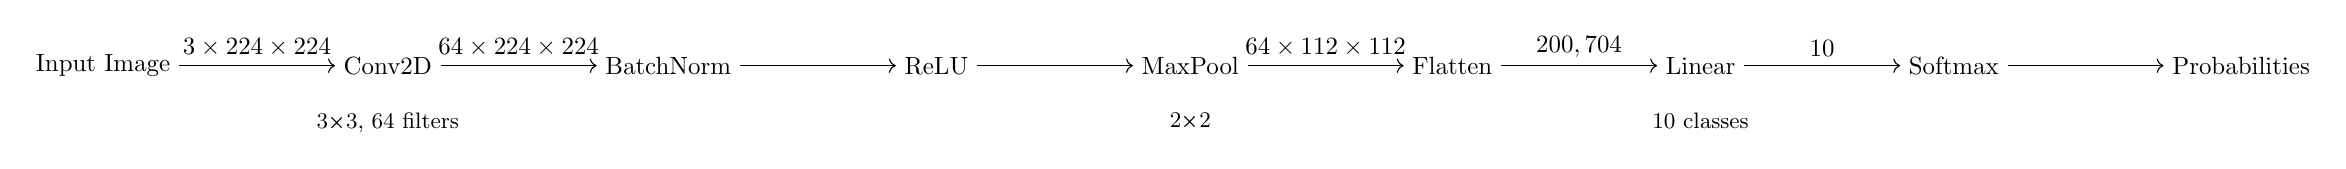
\begin{tikzpicture}[node distance=1.8cm and 2.2cm, auto, scale=0.9, transform shape]
    % Input
    \node (input) {Input Image};
    
    % Operations
    \node (conv) [right=of input] {Conv2D};
    \node (bn) [right=of conv] {BatchNorm};
    \node (relu) [right=of bn] {ReLU};
    \node (pool) [right=of relu] {MaxPool};
    \node (flatten) [right=of pool] {Flatten};
    \node (linear) [right=of flatten] {Linear};
    \node (softmax) [right=of linear] {Softmax};
    
    % Output
    \node (output) [right=of softmax] {Probabilities};
    
    % Edges
    \draw[->] (input) -- node[above] {\(3\times224\times224\)} (conv);
    \draw[->] (conv) -- node[above] {\(64\times224\times224\)} (bn);
    \draw[->] (bn) -- (relu);
    \draw[->] (relu) -- (pool);
    \draw[->] (pool) -- node[above] {\(64\times112\times112\)} (flatten);
    \draw[->] (flatten) -- node[above] {\(200,704\)} (linear);
    \draw[->] (linear) -- node[above] {\(10\)} (softmax);
    \draw[->] (softmax) -- (output);
    
    % Additional info
    \node [below=0.3cm of conv, font=\small] {3×3, 64 filters};
    \node [below=0.3cm of pool, font=\small] {2×2};
    \node [below=0.3cm of linear, font=\small] {10 classes};
\end{tikzpicture}
\end{center}

\subsection{Graph Optimization in Practice}

Modern deep learning compilers like XLA (Accelerated Linear Algebra) and TensorRT perform extensive graph optimizations:

\begin{enumerate}
    \item \textbf{Layer Fusion}: Combine Conv+BatchNorm+ReLU into a single kernel
    \item \textbf{Kernel Auto-tuning}: Test multiple implementations and select the fastest
    \item \textbf{Memory Planning}: Optimize tensor lifetimes to reuse memory
    \item \textbf{Quantization}: Insert quantization/dequantization nodes for INT8 inference
\end{enumerate}

\begin{lstlisting}[language=Python, caption=Graph optimization with PyTorch and TensorRT]
import torch
import torch_tensorrt

# Original model
model = MyNeuralNetwork().eval()

# Compile with TensorRT optimizations
optimized_model = torch_tensorrt.compile(
    model,
    inputs=[torch_tensorrt.Input((1, 3, 224, 224))],
    enabled_precisions={torch.float32, torch.float16},
    workspace_size=1 << 20
)

# The computational graph is now optimized for inference
\end{lstlisting}

\subsection{Key Takeaways}

\begin{itemize}
    \item A \textbf{computational graph} is the executable blueprint of a neural network
    \item It enables \textbf{automatic differentiation} through reverse-mode traversal
    \item \textbf{Graph optimization} significantly improves performance through fusion and kernel selection
    \item \textbf{Static graphs} prioritize performance and deployment; \textbf{dynamic graphs} prioritize flexibility and debugging
    \item The compiled computational graph is the actual artifact deployed to production environments
\end{itemize}

Without computational graphs, modern deep learning would be impossible—practitioners would need to manually derive and code gradients for every new architecture, an insurmountable task given the complexity of today's models.

\end{document}